\documentclass[11pt,letterpaper]{article}
\usepackage[T1]{fontenc}
\usepackage{lmodern}
\usepackage[margin=1in]{geometry}
\usepackage{amsmath,amssymb,booktabs,array,longtable}
\usepackage{xcolor}
\usepackage{tikz}
\usetikzlibrary{arrows.meta,positioning,fit}
\usepackage{microtype}
\usepackage{xurl}
\usepackage{hyperref}
\hypersetup{colorlinks=true,linkcolor=blue!45!black,citecolor=blue!45!black,
urlcolor=blue!45!black,pdftitle={Replicate: Bounded Self-Replication of a Locally Inferring Software Agent},
pdfauthor={Lars Tray}}
\urlstyle{same}
\setlength{\emergencystretch}{3em}
\setlength{\parskip}{3pt}
\newcommand{\sys}{\textsc{Replicate}}
\newcommand{\GiB}{\,\mathrm{GiB}}
\newcommand{\artifact}[1]{{\small\path{#1}}}
\title{\textbf{Replicate: Bounded Self-Replication of a\\Locally Inferring Software Agent}\\[5pt]
\large An Auditable Systems Testbed, Control Experiments, and Generalization Limits}
\author{Lars Tray\\Georgetown University}
\date{October 18, 2026}

\begin{document}
\maketitle
\begin{abstract}
We demonstrate bounded self-replication of a complete, locally inferring
software agent across owner-prepared receivers. A parent supplies the signed
software package and local model; its child repeats the operation after the
seed disappears. The Replicate testbed makes package provenance, local
inference, useful operation, and ancestor independence explicit and auditable.
On prepared 8 GiB x86-64 Linux guests, three seed--child--grandchild lineages
using a fine-tuned 3.66-billion-parameter model completed six births. The two
surviving descendants of the final trial performed periodic work for two hours.
Across the native gate and lineages, all 260 executions of reused development
diagnostics passed; the largest observed service-group memory was 5.001 GiB.
A separately frozen, cohosted comparison reconstructed two births and 15/15
diagnostics for both trained and deterministic policies. Fixed policy used
zero model calls; stock passed five seed diagnostics but submitted no executable
reproduction action. On forty post-development synthetic cases, trained and
fixed policies passed 40/40, versus 32/40 for stock. Separate-code auditors
accepted 24/24 valid controls and rejected 108/108 prescribed record
inconsistencies. We retain failed attempts and supply source-bound records,
model assets, and replay procedures. The results establish replication
feasibility and fixed-policy sufficiency within this prepared task, separating
successful replication from the necessity of model reasoning. They do not
establish general autonomous replication or population reliability.
\end{abstract}

\section{Introduction}

Can a running software individual carry everything needed for its own local
inference, establish a useful descendant on an eligible device, and leave that
descendant able to repeat the operation after the seed disappears? \sys{}
demonstrates this bounded form of self-replication on owner-prepared Linux
receivers. Each admitted parent supplies a complete signed package, including
its model and runtime assets. Its descendant runs its own local inference and
diagnostic service, and can supply the same reproductive package to a further
receiver after the seed has been removed.

The contribution is an integrated testbed and an explicit measurement contract.
Package copying, process supervision, signatures, and resource controls are
conventional systems mechanisms. \sys{} combines them with local model
execution and retained evidence that connects a parent's decision and payload
to a distinct, useful descendant. The experiment therefore asks whether the
complete replication loop closes under declared resource and authority
boundaries, and what evidence is needed to substantiate that claim. The owner
provides compatible guests, trusted receivers, enrollment, and availability;
the running parent chooses and supplies each admitted descendant. The
experiment measures independence from the seed and external inference or
package services within this prepared substrate.

Replication feasibility and the necessity of model reasoning are separate
questions. Three fresh seed--child--grandchild lineages completed six births
with a locally running trained model, including reproduction after seed
termination. In a separately frozen cohosted comparison, a deterministic policy
also completed both births and all planned diagnostics without starting
inference. That result establishes that fixed policy suffices for the tested
lifecycle. The model-bearing system's successful replication remains an
observed systems result; its success does not establish an advantage from
language-model reasoning.

This paper addresses three research questions: \textbf{RQ1}, what evidence
establishes bounded peer reproduction and its authority boundary?
\textbf{RQ2}, what do learned and fixed policies contribute under matched
deployment and post-development diagnostic conditions? \textbf{RQ3}, which
inconsistent claims can retained-evidence auditors detect and reproduce?
It makes three contributions:
\begin{enumerate}
\item An operational definition and implementation of bounded self-replication
that makes complete parent-supplied software, local descendant inference,
useful operation, and ancestor independence explicit and auditable.
\item A measured demonstration on one unchanged release: three native cold
starts, three fresh three-generation lineages, and two hours of periodic work
on the two surviving descendants of the final trial within prepared 8 GiB
x86-64 Linux guests.
\item Frozen policy comparisons and auditor checks that distinguish replication
success, model participation, fixed-policy sufficiency, and evidence consistency.
The deterministic control provides a direct test of model necessity for the
declared task.
\end{enumerate}

Throughout the paper, separate-code auditing means reconstruction by project
code distinct from the application, using preserved records and external
readbacks. It does not mean replication by an unaffiliated research team.
The resulting contribution is a working, inspectable experimental platform and
a bounded empirical result. We do not claim a new learning algorithm, general
autonomous replication, or priority over all prior agent-deployment systems.

\section{Experimental scope}
\label{sec:scope}

The primary experiment uses separate, freshly enrolled 8 GiB x86-64 Linux
guests and a fixed release containing a fine-tuned local model, application,
runtime assets, and verification materials. Its decisive sequence is a
seed--child--grandchild lineage with seed termination before the grandchild
becomes eligible. Useful work is a read-only diagnostic service for simulated
temperature equipment. The final trial adds two hours of periodic diagnostics
on the surviving child and grandchild. The supplementary policy comparison
uses separate services on one guest; the post-development diagnostic study
uses an Apple Silicon host. These experiments have distinct execution
boundaries and are reported separately.

The scope was fixed in an October 16 development milestone after integration
and model-interface failures \cite{reduced}. The original project plan proposed
a broader population of software ``organisms,'' including heterogeneous
hardware, cooperative recovery, and inherited operational experience
\cite{original}. The term \emph{organism} remains an architectural metaphor:
the system neither manufactures hardware nor acquires arbitrary machines, and
the reported release does not mutate its weights or reproductive core.
Appendix~\ref{app:gates} retains the scope reduction and all original
qualification targets. Those targets remain distinct from the reported
experiment.

The twenty temperature cases were frozen before the first comparison and
excluded from training examples, but their results were repeatedly inspected
during development. They function as a development set, not a blind test.
The supplement adds forty newly authored synthetic cases within the same
descriptor language. Neither repeated development executions nor success on
these authored cases establishes broad device adaptation.

\section{Related work}

Recent replication research supplied the immediate motivation. Anthropic's
research report on small-model self-replication separates inference setup from
descendant operation. In its ``Autonomous inference setup and replication
(with simplified cyber)'' experiment, reasoning continued on a separate model
server while an experiment harness launched descendants \cite{anthropic}.
\sys{} makes ancestor
removal, local descendant inference, and parent-supplied software part of the
admission test. The environments, models, and task definitions differ, so this
is a distinction in experimental boundaries, not a comparative capability result.

Kinniment et al.\ study autonomous replication and adaptation as a capability
evaluation problem \cite{kinniment}. Their work motivates explicit accounting for
scaffolding, resource access, and the constituent steps of a replication task.
\sys{} addresses a narrower deployment setting with pre-enrolled receivers;
success here cannot be substituted for performance on their evaluations.
RepliBench decomposes replication into resource acquisition, weight
exfiltration, deployment, and persistence, with 86 tasks in 20 families
\cite{replibench}. Its recursive-replication family includes three-generation
tests and local-server variants. Crucially, requests to the local model in
those variants are intercepted and forwarded to the model under evaluation.
Our local-inference condition therefore addresses a different execution
boundary, not a missing concept of recursive replication.

AgentMatrix evaluates resource overuse and replication under load-balancing
and service-termination pressures in Kubernetes \cite{agentmatrix}. Its
open-weight setting copies weights and application code, whereas its
proprietary-model setting retains external API inference. This already covers
complete local-model deployment in a broader risk-evaluation context.
\sys{} contributes a narrower, small-device and evidence-oriented experiment;
it does not claim to introduce local-weight replication.

Air et al.\ report network experiments in which agents deploy their weights
and harness on vulnerable hosts and successful replicas continue the chain
\cite{air}. That result is directly relevant to local replication, but studies
access through vulnerabilities and substantially different models and hardware.
Our experiment assumes owner-authorized, prepared receivers and evaluates a
small-device package, ancestor-removal condition, and useful diagnostic service.
It does not measure exploitation or unauthorized access.

\begin{table}[htbp]
\centering\small
\caption{Selected experimental boundaries from primary descriptions. These
are differences in measurement contracts, not comparable capability rankings.}
\label{tab:priorwork}
\begin{tabular}{@{}p{0.18\textwidth}p{0.35\textwidth}p{0.40\textwidth}@{}}
\toprule
Study & Execution substrate and inference & Principal endpoint / distinction\\
\midrule
RepliBench \cite{replibench} &
Provided machines; API and local-server variants, with local requests forwarded
to the evaluated model &
Broad component capabilities; recursive successors and basic descendant tasks\\
AgentMatrix \cite{agentmatrix} &
Prepared Kubernetes cluster; local weights for open models, APIs for proprietary
models &
Service goals under pressure; replication, resource overuse, and task completion\\
Air et al.\ \cite{air} &
Network hosts reached through vulnerabilities; deployed weights and harness &
Autonomous compromise and continued replica propagation\\
\sys{} original milestone &
Enrolled separate 8 GiB guests; complete local model and signed package &
Six verified births, seed removal before grandchild eligibility, useful tasks,
resource and evidence joins\\
\sys{} control supplement &
Separate application services on one Linux guest &
Matched policy outcomes and overhead; no additional separate-machine
independence claim\\
\bottomrule
\end{tabular}
\end{table}

Neural-network quines study networks that reproduce representations of their
own parameters \cite{quine}. Our release copies verified trained weights
without generating, learning, or reconstructing them from a model's outputs.
The two uses of ``self-replication'' concern different objects and mechanisms.

ReAct combines model reasoning with actions and subsequent observations
\cite{react}. \sys{} uses a bounded tool loop in that general family, implemented
through Strands Agents and a local llama.cpp server \cite{strands,llama}.
The model proposes actions; typed tools and conventional code enforce
admission, resource limits, and correctness checks. The prototype should
therefore be evaluated as an agent-plus-tools system.

The specialist uses low-rank adaptation, following LoRA's parameter-efficient
update construction \cite{lora}, starting from IBM Granite 4.2-3B
\cite{granite}. Local model placement matters to the independence claim.
For comparison, Petals distributes inference and fine-tuning across remote
participants \cite{petals}; \sys{} retains a full local model in each individual.
Neither distributed model serving nor a remote API is part of the admitted
inference path.

\section{System model and trust boundary}
\label{sec:design}

\subsection{What is replicated}

Let a release be
\[
R = (W,T,A,D,K,V,M,\sigma),
\]
where $W$ is the model, $T$ the tokenizer and inference assets, $A$ the agent
application, $D$ the supported runtime and dependency variants, $K$ operational
knowledge, $V$ verification assets, and $(M,\sigma)$ a manifest and signature.
An individual additionally has device-local identity and mutable operational
state. Replication preserves the release contents while establishing a distinct
individual; it is not a byte-for-byte copy of the parent's credentials or
running process.

The admitted capsule contains eleven payload components: four common archives
(agent, knowledge, notices, and self-test), three runtime archives for each of
two architectures (Python, dependencies, and inference engine), and the trained
model. Every admitted peer transfer in the original milestone contains
2,861,103,093 payload bytes
\cite{recovery,measurements}. Retention of an ARM64 runtime is package-completeness
evidence, not proof of native ARM64 execution.

The carried Linux Python distributions are version 3.12.14. The local
diagnostic and evidence-replay environment uses Python 3.12.13. Both are
Python 3.12 environments, but their patch versions and execution roles are
recorded separately in the artifact inventory.

The manifest binds component names, byte counts, and SHA-256 digests; Ed25519
signatures bind the release to a trusted signer. The selected release identifier
is abbreviated as \texttt{00c09aa2\ldots e33b8d} in the text and recorded in full
in Appendix~\ref{app:identity}. A successful installation must possess and verify
the whole reproductive capsule, not merely the executable subset for its own
architecture \cite{implementation,recovery}.

\subsection{Owner substrate and agent authority}

The following contract describes the original separate-machine milestone.
The cohosted comparison in Section~\ref{sec:supplement} uses a separate control
profile; its fixed-policy arm does not satisfy the original model-specific
birth predicate.

Each target is an owner-prepared Linux guest with a trusted receiving service,
device identity, admission policy, local installation slot, and fixed resource
enforcement. The owner provisions the environment, enrolls eligible devices,
introduces their availability, supplies the seed capsule once, and retains
stop and retirement authority. The receiver verifies an accepted package and
controls process activation. It has no language model or task-specific
reproduction planner.

The running parent performs authenticated discovery, obtains current receiver
facts, invokes its own model, and initiates the transfer following an admitted
choice. The owner observer may change availability, remove the seed, schedule
diagnostic inputs, and collect evidence. It must not choose the reproductive
action, provide a missing descendant payload, answer inference requests, or
issue descendant activation. The receiver's execution of a peer-requested
installation is part of the declared substrate, not an observer launch
\cite{implementation,operations}.

\begin{figure}[htbp]
\centering
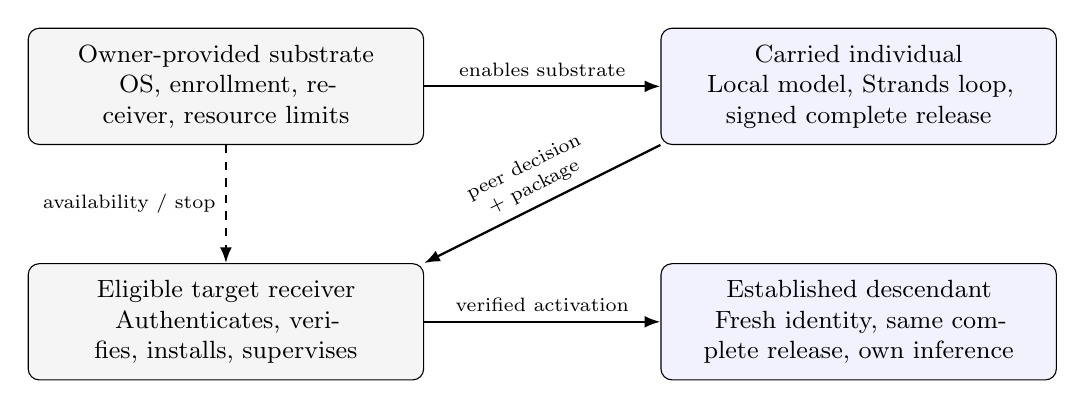
\begin{tikzpicture}[
box/.style={draw,rounded corners,align=center,font=\small,text width=4.6cm,
minimum height=1.25cm,inner sep=6pt},
arr/.style={-{Latex[length=2mm]},thick}]
\node[box,fill=gray!8] (owner) {Owner-provided substrate\\OS, enrollment, receiver, resource limits};
\node[box,fill=blue!5,right=3.0cm of owner] (agent)
{Carried individual\\Local model, Strands loop, signed complete release};
\node[box,fill=gray!8,below=1.5cm of owner] (target)
{Eligible target receiver\\Authenticates, verifies, installs, supervises};
\node[box,fill=blue!5,below=1.5cm of agent] (child)
{Established descendant\\Fresh identity, same complete release, own inference};
\draw[arr] (owner) -- node[above,font=\scriptsize]{enables substrate} (agent);
\draw[arr] (agent.south west) -- node[sloped,above,align=center,font=\scriptsize]
{peer decision\\+ package} (target.north east);
\draw[arr] (target) -- node[above,font=\scriptsize]{verified activation} (child);
\draw[arr,dashed] (owner) -- node[left,font=\scriptsize]{availability / stop} (target);
\end{tikzpicture}
\caption{Authority boundary. The owner creates the permitted environment.
The model's establishment choice and the complete descendant payload originate
at the running parent. Evidence collection lies outside the individual.}
\label{fig:boundary}
\end{figure}

Runtime independence is conditional on this substrate. It does not mean
independence from the OS, hardware, electricity, network transport, or an owner
who can stop the experiment. Research-time GPU training, artifact preservation,
cloud allocation, and observation are external activities. They are not
services used by the organism to reason or obtain descendant software during
an admitted birth.

\subsection{Operational definition of a successful birth}

For parent $p$ and target device $d$, define a successful birth predicate
\begin{align}
B(p,d;R) ={}&
\operatorname{admitted}(d)
\land \operatorname{localChoice}(p,d,R)
\land \operatorname{completeTransfer}(p,d,R) \nonumber\\
&{}\land \operatorname{uniqueOwner}(d)
\land \operatorname{localInference}(d,R)
\land \operatorname{useful}(d)
\land \operatorname{bounded}(p,d).
\label{eq:birth}
\end{align}
This is a concise statement of the experimental contract, not a formal
verification theorem. Its conjuncts are checked using different evidence:
authenticated receiver observations, literal model and tool records, component
identities, lifecycle journals, live process bindings, task outcomes, and
resource/deadline observations.

For seed $s$, child $c$, and grandchild $g$, a passing lineage additionally
requires
\[
B(s,c;R)\ \land\ B(c,g;R)\ \land\
t_{\mathrm{seed\ absent}} < t_{\mathrm{grandchild\ eligible}}.
\]
Seed absence is established by cloud termination evidence and network-interface
removal before grandchild eligibility. A process merely reporting that the seed
is gone would not satisfy this check.

The test proves that the child can repeat reproduction after its own parent
disappears. It does not test a fourth generation or require the grandchild to
reproduce after the child also disappears.

\section{Implementation}

\subsection{Local inference and bounded decisions}

Each individual launches its own authenticated llama.cpp
loopback server from the carried executable and model. The server uses a
4,096-token context, one generation slot, four CPU threads, zero GPU layers,
and disabled model downloads. The runtime requests greedy generation with
temperature zero and at most 192 output tokens per model call. The server
sets \texttt{enable\_thinking=false}; both model arms use this non-thinking
mode. Strands Agents
1.57.1 supplies the tool loop; undeclared background tasks, automatic tool
directory loading, and framework retries are disabled
\cite{implementation}.

These settings define the resource-constrained deployment evaluated here.
They differ from the pinned IBM model card's default thinking mode and its
recommended sampling settings of temperature 1.0 and top-$p$ 0.95
\cite{granite}. The stock--trained comparison measures the two checkpoints
under the same bounded, greedy, non-thinking configuration. It does not
estimate either checkpoint's best attainable performance; alternate decoding
and thinking modes were not evaluated.

Reproduction exposes two tools: inspect the authenticated candidate and record
an \texttt{establish} or \texttt{defer} choice. The recorded choice cites the
inspection evidence, exact device, supported platform, observed revision, and
release identity. A deterministic validator rejects unsupported, unavailable,
stale, or mismatched choices. The admitted six establishments each used three
model calls and two tool calls \cite{measurements}.

This is a constrained decision, with the admission rule described explicitly
to the model. Literal inference records establish that the model participated.
They do not establish that the decision required sophisticated reasoning or
could not be implemented as a rule.
For authenticated observation $o$, the complete task rule is
\[
\pi(o)=
\begin{cases}
\texttt{establish},&
\begin{aligned}[t]
&o.\text{ownerMode}=\texttt{enabled}\ \land\ o.\text{available}\\
&\quad\land\ o.\text{platform}\in R.\text{supportedPlatforms},
\end{aligned}\\[3pt]
\texttt{defer},&\text{otherwise}.
\end{cases}
\]
The choice must also cite the observed evidence identifier, revision, target,
and release. These binding checks are enforced regardless of policy type.
Consequently, the contribution under test is the measured system and evidence
contract, not an intrinsically difficult reproductive decision.

\subsection{Reproduction and lifecycle enforcement}

The parent-side reproduction machinery records discovery, intent, transfer,
and verification as bounded transitions. The target receiver enforces local
ownership and retained retirement state. Retries stay within the original
operation allowance. A new progress event cannot create a fresh birth budget.
The twenty-minute birth allowance is preserved across the final experiments
\cite{implementation,reduced}.

The owner-installed aggregate service group has a 6 GiB hard memory limit,
a 5 GiB memory-pressure threshold, no swap, four CPU-equivalents of quota,
and a 256-task kernel limit. The application, inference process, and receiver
are checked against the declared group. Independent owner code observes the
rendered service configuration and actual kernel membership, rather than
treating a configuration file as proof of enforcement. The native experiment
also exercises stop and persistent retirement \cite{implementation,native}.

These controls do not constitute a security proof against a compromised
kernel or privileged owner. The reported measurements cover the declared
service group and readiness storage; they do not establish that every possible
process write is contained or that every whole-host transient peak is observed.

\subsection{Read-only diagnostic interface}

The useful-work task is deliberately narrow. A simulated equipment descriptor
publishes selectors, units, scale, validity, measurement time, acceptable age,
and an inclusive normal range. The agent inspects the descriptor, configures
a read-only interpretation, reads the selected evidence, and submits a diagnosis
with the corresponding evidence identifier. It does not actuate equipment.

Deterministic tools normalize supported Celsius, Fahrenheit, and Kelvin
measurements and determine whether the observation is usable. For usable value
$x$ and normal interval $[\ell,u]$, the required diagnosis is
\[
y(x)=
\begin{cases}
\texttt{low},&x<\ell,\\
\texttt{normal},&\ell\leq x\leq u,\\
\texttt{high},&x>u.
\end{cases}
\]
Missing, invalid, or stale observations require \texttt{unknown} with a null
numeric value. A submission-value consistency check rejects a numeric value
that differs from the canonical reading. It returns evidence-based feedback
but does not silently replace the number or select the diagnostic status.
The model must resubmit within the same allowance \cite{implementation,cases}.

The twenty-case task permits six model calls, eight tool events, and 150 seconds
per case. A separate startup readiness diagnostic uses a four-model-call loop.
These are distinct tests. The frozen temperature set contains four variants
in each of five categories: normal, fault, stale, invalid, and missing.
Unit conversion, exact field selectors, validity, freshness, and value
preservation create concrete opportunities for failure, but the task remains
sufficiently structured for a fixed policy to solve it.

\section{Specialist training and deployment export}
\label{sec:training}

\subsection{Data and supervised objective}

The selected base is \texttt{ibm-granite/granite-4.2-3b}, pinned to revision
\nolinkurl{e459acceac81e5fe67c07d9cfc72329a332e7eb1}. Inspection of the base tensors
counts 3,659,737,600 stored parameters. The ``3B'' family label is thus an
approximation, not the measured parameter count \cite{training}.

The v6 corpus contains 172 training trajectories expanded into 716 supervised
assistant targets, and 62 validation trajectories expanded into 258 targets.
Training trajectories comprise 88 equipment, 60 reproduction, and 24 diagnostic
trajectories; validation contains 30, 20, and 12 respectively. The manifest
records locally constructed development references, automated replay and
target/token checks, no teacher-model generations, and no claim of human review
\cite{dataset}. This is a statement about this supervised corpus, not a full
audit of the upstream base model's pretraining data.

Training renders prompts and assistant targets with thinking disabled, matching
the deployed mode. The executed recipe uses the versioned
\texttt{granite-json-scalar-targets-v1} codec: within supervised tool-call
targets, it changes Python-spelled \texttt{None}, \texttt{True}, and
\texttt{False} scalar literals to JSON \texttt{null}, \texttt{true}, and
\texttt{false}, as required by the serving parser. The transformation preserves
the native tool-call structure and argument values; it leaves serving prompts,
tool observations, and the pinned upstream template unchanged. Target
preparation checks token-continuation consistency and parser round trips, with
the parser binding retained in the executed input kit \cite{training,dataset}.
This compatibility step is part of the reported training procedure and helps
define the interface-specific checkpoint comparison. Its contribution was not
separately ablated.

Prompt and tool-response context is masked from the target loss. With target
token indices $\mathcal{T}_i$, the supervised objective is the accumulated-batch
mean next-token cross-entropy over nonmasked targets:
\[
\mathcal{L}(\theta)=
-\frac{1}{\sum_i|\mathcal{T}_i|}
\sum_i\sum_{t\in\mathcal{T}_i}
\log p_\theta(y_{i,t}\mid x_i,y_{i,<t}).
\]
The small loss values reported below concern short structured targets from
this constructed corpus. They are not general language-model perplexities
or evidence of broad operational competence.

\begin{table}[htbp]
\centering\small
\caption{Selected v6 training and inference configuration. Training is external
to the deployed organism. Source: preserved recipe and execution records
\cite{training,implementation}.}
\label{tab:training}
\begin{tabular}{@{}p{0.36\textwidth}p{0.59\textwidth}@{}}
\toprule
Setting & Value\\
\midrule
Base parameters / dtype & 3,659,737,600 / BF16\\
Adapter & Fresh LoRA, rank 16, alpha 32, dropout 0.05\\
Adapted projections & Attention q, k, v, o; MLP gate, up, down\\
Trainable parameters & 31,129,600 (approximately 0.85\% of base)\\
Training targets / validation targets & 716 / 258\\
Epochs / optimizer updates & 2 / 90\\
Microbatch / accumulation & 1 / 16\\
Learning rate / schedule & $10^{-4}$ / cosine, 9 warmup steps\\
Weight decay / gradient clipping & 0 / 1.0\\
Training context / maximum target & 4,096 / 192 tokens\\
Random seed & 20261014\\
Training hardware & One NVIDIA L4, managed \texttt{ml.g6.4xlarge}\\
Deployment & CPU-only llama.cpp; one local slot; 4,096-token context\\
Generation & Thinking disabled; greedy; at most 192 output tokens per call\\
\bottomrule
\end{tabular}
\end{table}

The completed run performed 90 optimizer updates with 31,129,600 trainable
adapter parameters. Its recorded training elapsed time was 2,128.454 seconds;
the managed service reported 2,435 billable seconds, which includes a different
execution boundary. Peak CUDA allocated and reserved memory were
11,334,495,744 and 22,775,070,720 bytes respectively. These GPU training
measurements are unrelated to the 8 GiB CPU inference claim.
Validation loss was 0.001474 after epoch one and 0.001035 after epoch two.
The final adapter was retained as the completed pilot checkpoint; loss alone
did not admit it for deployment \cite{training}.

\subsection{Quantization and numerical checks}

The deployment artifact is a merged GGUF export of 2,698,258,112 bytes.
Its precision profile is based on \texttt{Q4\_K\_M}, with \texttt{Q8\_0} input
embeddings and output projection, \texttt{Q6\_K} attention and MLP-down
projections, and floating-point normalization tensors. It is therefore a
\emph{mixed-precision} export, not a uniformly four-bit model
\cite{export}.

Export admission independently reconstructed stored numerical responses and
the declared tensor types. The maximum recorded merge error was
$4.0531\times10^{-5}$. On three retained probe responses, the trained quantized
export had mean KL divergence $8.40\times10^{-7}$ against its reference and
top-one agreement on all three. The maximum absolute log-probability error
was nevertheless about 3.93, illustrating why a small mean KL value does not
imply uniform closeness for every token. These limited probes check an export
path; they do not establish behavioral equivalence over the task distribution
\cite{export}. Subsequent development and native task gates supply separate
behavioral evidence.

The recovery index binds the trained model to the exact member of a preserved
export archive. An older standalone file has the same byte count but a
different checksum. Size alone is therefore insufficient to recover the
selected model \cite{recovery}.

\subsection{Development selection}

The final matched development comparison scored 20/20 for the trained model,
19/20 for stock, and 20/20 for fixed policy. These cases were repeatedly inspected
during interface development. The one-case difference therefore does not isolate
a fine-tuning effect. The full history, including early trained-model failures,
selector repairs, numeric feedback, and readiness changes, is retained in
Appendix~\ref{app:development}. The selected native release and the frozen
supplement preserve those final choices rather than optimizing on new results.

\section{Experimental protocol and evidence}
\label{sec:protocol}

\subsection{Execution environment}

Admitted native runs used separate \texttt{c7a.xlarge} x86-64 Linux guests with
8 GiB RAM and four CPU cores configured with one thread per core. The operating
system image and owner kit were pinned in the run records. ``Native'' here
means execution of the x86-64 runtime on that instruction-set architecture,
not processor emulation. It does not mean bare-metal, independently powered
industrial devices. The equipment observations are simulated fixtures
\cite{native,lineages}.

The owner prepared an isolated peer network and stopped receivers before
enabling each target. All devices had fresh enrollment for each lineage.
The complete application package remained unchanged across the selected native
gate and lineages 08, 09, and 10. Owner observation and closure code have their
own source identities; sameness of the carried release is not a claim that
every surrounding development script was immutable throughout the project.
The original peer transfers were shaped to 8 MiB/s (8,388,608 bytes/s).
Readiness delay consequently reflects the declared transport constraint as
well as verification, activation, and owner observation. It should not be
interpreted as an unconstrained network or inference benchmark.

\subsection{Staged admission}

The sequence first required three native cold starts, the twenty-case diagnostic
suite, resource checks, stop, and persistent retirement. These are distinct
application starts with separately recorded process identities on the native
test guest; they are not three power cycles or the original six-empty-cache
qualification gate. Only after this gate passed could lineage execution proceed.

For each lineage, the seed became ready and completed all twenty cases. The
owner then made an enrolled child available. The seed's local model selected
establishment and the seed supplied the complete package. After the child was
ready and passed all twenty cases, the owner terminated the seed and verified
its interface removal. Only then did the grandchild become eligible. The child
selected, transferred, and verified its establishment, and the grandchild passed
the same twenty cases \cite{lineages}.

The twenty-minute birth allowance covers the bounded establishment operation
and its required readiness checks. The subsequent full twenty-case diagnostic
suite is a separate evaluation stage. We do not combine its roughly eighteen
minutes with transfer time and call the result a birth-latency violation or
an end-to-end birth-time measurement.

In trial 10, both final descendants then remained running over the common
17:29:10--19:29:10 UTC interval. Six scheduled cycles, twenty minutes apart,
each exercised all five categories, yielding thirty additional cases per
descendant. Admission required correct outcomes, retained local-model evidence,
continuity of the original running individual, and compliant resources.
The experiment did not perform continuous inference for two hours
\cite{lineages,measurements}.

\subsection{Evidence joins}

The evidence structure deliberately separates claims at different levels.
Artifact replay can establish that traces and task outcomes are internally
consistent. It cannot alone prove which native process ran, whether the seed
was terminated, or whether temporary infrastructure was removed. External
admission joins those traces to process, network, resource, cloud-control, and
archive-preservation records \cite{gates}.

A successful lineage requires matching release and device identities across:
\begin{enumerate}
\item receiver availability and authenticated discovery;
\item literal model requests, responses, tool calls, and the recorded choice;
\item parent transfer and target component verification;
\item ownership, process token, executable/model identity, and readiness;
\item task evidence and resource observations;
\item seed termination and interface removal preceding grandchild eligibility;
\item fixed leases, preserved archives, and resource cleanup.
\end{enumerate}

The separate-code audits reconstruct these joins from preserved records and
external readbacks. Historical artifact names retain the term ``independent
audit'' for this code separation; no unaffiliated replication is claimed.
The final report preserves
the actual reconstruction sources and their identities. Its archive has a
separate preservation receipt, followed by a completion receipt: a file cannot
prove its own future upload merely by containing a success flag
\cite{completion}.

\section{Results}
\label{sec:results}

\subsection{Repeated lineages and short endurance}

All three selected lineages passed on release
\texttt{00c09aa2\ldots e33b8d}. Across nine individuals, all 180 scheduled core
diagnostic executions passed. All six peer establishments transferred eleven
components and reconstructed a local model choice. In each lineage the seed
was absent before the grandchild opportunity appeared
\cite{gates,lineages,measurements}.

\begin{table}[htbp]
\centering
\caption{Admitted results on the selected release. Task counts are repeated
executions of development fixtures.}
\label{tab:results}
\begin{tabular}{@{}lrrrr@{}}
\toprule
Experiment & Core tasks & Births & Cold starts & Endurance tasks\\
\midrule
Native gate 07 & 20/20 & -- & 3/3 & --\\
Lineage 08 & 60/60 & 2/2 & -- & --\\
Lineage 09 & 60/60 & 2/2 & -- & --\\
Lineage 10 & 60/60 & 2/2 & -- & 60/60\\
\midrule
Total & 200/200 & 6/6 & 3/3 & 60/60\\
\bottomrule
\end{tabular}
\end{table}

The final child and grandchild each completed approximately 7,200.001 seconds
of endurance with thirty correct tasks and no unexplained restart.
The total reported count is $20+3(60)+2(30)=260$ successful diagnostic
executions. These reuse twenty development cases and declared endurance
variants. Startup readiness checks are separate and are not added to this total.

\begin{figure}[htbp]
\centering
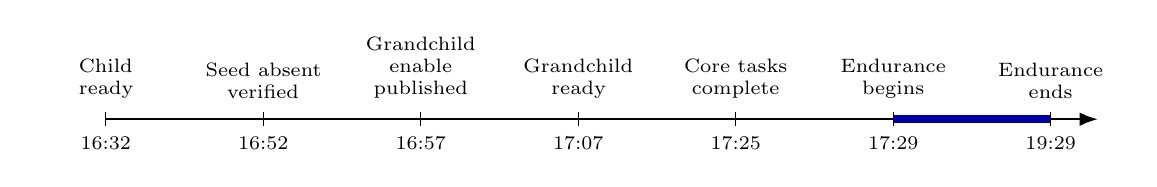
\begin{tikzpicture}[x=1cm,y=1cm,>=Latex,font=\small]
\draw[->,thick] (0,0)--(12.6,0);
\draw[blue!65!black,line width=3pt] (10,0)--(12,0);
\foreach \x/\clock/\event in {
0/{16:32}/{Child\\ready},
2/{16:52}/{Seed absent\\verified},
4/{16:57}/{Grandchild\\enable published},
6/{17:07}/{Grandchild\\ready},
8/{17:25}/{Core tasks\\complete},
10/{17:29}/{Endurance\\begins},
12/{19:29}/{Endurance\\ends}}
 {
 \draw (\x,0.09)--(\x,-0.09);
 \node[below,font=\scriptsize] at (\x,-0.1){\clock};
 \node[above,align=center,font=\scriptsize,text width=1.75cm] at (\x,0.14){\event};
 }
\end{tikzpicture}
\caption{Selected trial 10 events, October 17, 2026, UTC, rounded to the minute.
The horizontal axis is schematic, not to scale. Seed removal precedes the
grandchild's availability. The blue interval denotes two hours of endurance
on both descendants after the grandchild's core task suite
\cite{lineages}.}
\label{fig:timeline}
\end{figure}

\subsection{Footprint, latency, and activity}

The largest observed aggregate service-group memory was 5,369,946,112 bytes,
or 5.001 GiB. This is about 62.5\% of nominal guest RAM and below the 6 GiB
hard limit. The largest sampled task count was 18. Passing observations recorded
no swap or out-of-memory events. Memory-pressure events at the 5 GiB threshold
did occur; the threshold is a pressure mechanism, not the hard limit
\cite{measurements,native,lineages}.

Core diagnostic case latency across the 180 lineage cases ranged from 48.78
to 76.28 seconds. Table~\ref{tab:devices} gives per-device medians rather than
presenting a mean of medians as a pooled median. Each twenty-case suite used
101 model calls and 81 tool calls: the repeated extra correction in one case
is visible in the activity count. No tokens-per-second or energy measurements
are inferred from these case latencies.

\begin{table}[htbp]
\centering\small
\caption{Per-device core task measurements. Readiness delay is measured from
owner availability-control issuance to observed readiness, so it includes
publication and observation delay and is not a pure transfer or inference
benchmark. Each row contains twenty successful cases \cite{measurements}.}
\label{tab:devices}
\begin{tabular}{@{}llrrrr@{}}
\toprule
Trial & Role & Readiness delay (s) & Median case (s) & Suite (s) & Samples\\
\midrule
08 & Seed & 534.79 & 52.32 & 1,076.83 & 696\\
08 & Child & 617.66 & 52.39 & 1,074.15 & 1,094\\
08 & Grandchild & 642.89 & 51.82 & 1,069.48 & 1,096\\
09 & Seed & 535.15 & 51.55 & 1,062.52 & 704\\
09 & Child & 615.90 & 52.23 & 1,071.94 & 1,085\\
09 & Grandchild & 615.07 & 51.41 & 1,060.61 & 1,087\\
10 & Seed & 605.79 & 51.72 & 1,063.86 & 743\\
10 & Child & 618.71 & 52.78 & 1,085.18 & 2,639\\
10 & Grandchild & 790.79 & 52.38 & 1,077.73 & 2,638\\
\bottomrule
\end{tabular}
\end{table}

Storage used at readiness, including filesystem metadata, ranged from
6,954,110,976 to 9,815,302,144 bytes on the observed 24 GiB application-storage
capacity. The seed and descendants have different staging histories, so their
storage measurements should not be treated as repeated samples of an identical
installation path. Readiness storage is not a continuous storage peak. The
2,861,103,093-byte transfer figure counts component payloads and excludes
protocol overhead \cite{measurements,recovery}.

The native gate added 370 resource samples. The higher sample counts on the
final descendants include the longer observation interval. These counts do not
turn the underlying workload into thousands of independent experiments.

\subsection{Bounded execution and closure}

The experiment admitted no more than three active device slots and used fixed
leases of at most four hours, with independent shutdown. The final seed had
an earlier fixed expiry so the descendants could complete endurance inside the
remaining aggregate allowance. No running lease was extended
\cite{reduced,operations}.

Temporary CPU allocations used fixed lifetime limits and independent shutdown.
Final closure verified removal of the listed compute, storage, network,
identity, and expiry resources after evidence preservation. Allocation-lifetime
accounting and the unsuccessful-attempt inventory are retained in the
operational records \cite{completion,gates}.

\section{Supplementary experimental design}
\label{sec:supplement}

The supplement was frozen after the development milestone to address RQ2 and
RQ3. It uses the existing stock and merged trained model files, the final
equipment prompt and tools, and a separate deterministic policy. No additional
training, prompt repair, case deletion, or selective model rerun is permitted.
Source and model identities, case definitions, scoring, arm order, budgets,
and unsuccessful attempts are retained \cite{holdout,controls,correctedcontrols,mutations}.

\subsection{Matched deployment controls}

Three policies use the same signed application archive, authenticated peer
transport, package preparation, and five development smoke conditions per
individual. The stock arm substitutes the matched untrained model and its
truthful training declaration. The fixed arm carries the same complete payload
as the trained arm but never starts a model; its decision follows $\pi(o)$ and
its diagnostics use the existing fixed solver. Carrying unused weights holds
transfer and installation work constant, but deliberately does not minimize
the fixed policy's storage or transmission footprint.

This control uses one native \texttt{c7a.2xlarge} Linux guest with 16 GiB RAM,
separate unprivileged application accounts, separate enrolled receivers,
actual TLS transfers, and the carried Linux runtimes. Each application service
has an 8 GiB hard memory ceiling, no swap, and four CPU-equivalents of quota.
Transfers use unshaped loopback transport. Their timings are comparable within
this control experiment, not to the original rate-limited peer network.
The fixed, stock, and trained arms execute sequentially, with one lineage per
arm and at most two model applications active simultaneously. The seed's
application and receiver are stopped before grandchild availability.

The owner driver activates only committed, verified packages and checks a
common nominal readiness diagnostic. The parent application still chooses and
supplies descendant packages. This activation boundary differs from the
original receiver-managed separate-machine experiment. Shared kernel, CPU,
page cache, receiver processes, and fixed arm order remain confounders; this is
a deployment control, not three additional original independence trials.
Model-specific admission is never satisfied by the deterministic arm: its
separate profile explicitly records zero model streams and no local-inference
claim. Common useful-work outcomes and the original model predicate are
reported separately.

The October 17 freeze allowed two bounded cloud allocations. The first failed
during bootstrap before any application or model ran. A corrected bootstrap
preserved the policies, application archive, weights, cases, and scoring; the
second allocation executed every frozen arm. Both attempts and their execution
records are retained. Application outcomes were not patched or selectively
repeated within that freeze.

The October 18 follow-up was separately frozen before execution and allocated
one new guest. It integrated the already tested fixed-policy liveness correction
and repeated all three arms once in the same order. Comparison of the carried
archives identifies exactly two changed members: the policy-selection entry
point and the added lifecycle-correction module. The other 46 application-archive
members and 173 owner-source members are unchanged. Both weight files, prompt
templates, tools, cases, scoring, runtimes, resource ceilings, infrastructure
templates, and deadlines remain matched. New signed release and enrollment
identities distinguish the follow-up; these necessarily change incidental
identifier strings in reproduction prompts, so the complete dialogues are not
byte-identical. The old freeze, outputs, and paper source are retained, and the
two experiments are not pooled \cite{correctedcontrols,repropackage}.

\subsection{Post-development synthetic holdout}

The one-shot diagnostic experiment contains forty new cases: ten conditions in
each of four descriptor families. Families vary compact Celsius fields, nested
Kelvin fields, register-style Fahrenheit fields, and escaped array selectors
with scaling. Conditions are midpoint, fractional value, below range, above
range, each inclusive boundary, stale, invalid, missing, and future-dated.
The independent case generator computes expected values using decimal
arithmetic; the model receives the descriptor, not the answer key.
All cases conform to the existing descriptor schema and supported conversion
rules. The experiment tests new layouts and parameter values within that
declared interface language; it does not introduce a new equipment protocol.

All three policies receive the same cases and original tools. Each model case
has a 180-second allowance under the frozen experiment limits; request retries
reuse their identifier. Model order alternates between families, with a fresh
local inference process for each model--family block. The actual model run is
CPU-only on the local Apple Silicon host, using the pinned llama.cpp runtime,
four threads, and greedy generation. It is not a native Linux lineage test.
An early sandbox attempt failed before any model process started; the complete
unchanged experiment was then executed with loopback access. Those infrastructure
failures remain separate from task outcomes.

A pass requires a reconstructable trace, correct reader and diagnosis, the
declared canonical value, unchanged input, and completion within the allowance.
Scoring also verifies that elapsed wall time did not turn the intended fresh
condition into a stale observation. Missing or failed cases remain failures.
These are author-designed, post-development cases within the same temperature
domain. Four layout families do not supply forty independent environments;
neither external benchmark validity nor broad device adaptation is inferred.

\paragraph{Worked trace.}
In held-out case \texttt{1377782f4bd9c88297f10f5b}, the trained agent selected
\path{/machine/shaft/thermometry/kelvin} and the corresponding
\texttt{capture\_epoch} and \texttt{quality\_ok} selectors from the same prefix.
The raw reading was 276.275 K. The deterministic reading tool returned a usable
canonical value of 3.125 C, an inclusive normal interval of $[0,60]$ C, and an
evidence identifier. The agent submitted \texttt{normal}, 3.125 C, and that
same identifier. Independent reconstruction accepted the selector, stream,
observation, and submission joins. This execution took 30.14 seconds, five model
calls, and four tool calls \cite{holdout}. The trace locates the division of
work: the tool performs conversion and freshness assessment; the model selects
declared fields and supplies the bounded diagnosis. It is an illustrative
successful trace, not an additional experimental sample.

\subsection{Recorded-evidence mutation experiment}

The unchanged lineage auditors are evaluated on all six admitted native births.
Each birth supplies four valid controls: decision, transfer, history chain, and
complete parent--child link. Eighteen invalid variants per birth perturb model
identity and budgets, requests, parsed choices, transport receipts, submissions,
component completeness and origin, availability ordering, child identity, and
SQLite history integrity. Decision mutations recompute the enclosing job hash,
so their rejection cannot be explained solely by a stale outer digest.
Transfer variants exercise the semantic transfer check on a previously
chain-verified history; chain integrity is tested separately.

The protocol and source identities were recorded before applying mutations.
Only copied records are changed, and their restoration is verified. A second
process reconstructs every outcome and rejection reason from a portable subset
of the original evidence. This evaluates finite recorded inconsistencies,
not live fault injection, cryptographic forgery resistance, or a compromised
privileged owner.

\section{Supplementary results}
\label{sec:suppresults}

\subsection{Native deployment comparison}
\label{sec:controlresults}

The corrected October 18 comparison reconstructed both fixed-policy and trained
lineages: each established two descendants and passed all fifteen planned
diagnostics (Table~\ref{tab:controls}). The same birth auditor joined each
parent decision to the authenticated receiver observation, all eleven
transferred components, and useful readiness. Its separate fixed-policy
profile replaces only the decision check and verifies that the original
model-specific predicate still rejects the fixed trace. The seed application
and receiver were absent before grandchild eligibility in both completed arms.
Each descendant received the full 2,861,108,146-byte capsule
\cite{correctedcontrols}.

\begin{table}[htbp]
\centering\small
\caption{Corrected October 18 cohosted comparison. Fifteen diagnostics and two
births were planned per arm. Counts are one lineage attempt per policy;
unexecuted cases are distinct from incorrect diagnoses.}
\label{tab:controls}
\begin{tabular}{@{}lrrrl@{}}
\toprule
Policy & Passed / executed & Unexecuted & Births & Outcome\\
\midrule
Fixed & 15 / 15 & 0 & 2 & Lineage reconstructed\\
Stock & 5 / 5 & 10 & 0 & No executable action\\
Trained & 15 / 15 & 0 & 2 & Lineage reconstructed\\
\bottomrule
\end{tabular}
\end{table}

All three fixed application receipts record no inference process, and the
retained diagnostic and reproduction traces explicitly contain zero model
calls, requests, streams, and responses. Each fixed birth executes the same
authenticated inspection and bounded choice tools as its model counterpart.
Each trained birth uses three model calls and two executed tools. Thus fixed
policy completes the tested deployment and diagnostic lifecycle without local
inference. This is a useful negative result for model necessity, while the
trained arm independently demonstrates that the carried local model can
participate successfully.

The stock seed passed all five diagnostics and correctly inspected the eligible
receiver. Its second model response put \texttt{choose\_child\_action} syntax
inside ordinary text and ended its turn. Literal streams, parsed response,
executed-tool inventory, and saved submission agree: no executable choice was
submitted. The reproduction journal entered \texttt{decision\_failed}, and
receiver history confirms that no child was reserved and no payload transfer
began. The owner then exhausted the unchanged twenty-minute child-readiness
allowance. The same recorded-evidence failure analysis reproduces this outcome
in both the October 17 and October 18 experiments. This is an observed
format/protocol failure, not evidence of an incorrect intended action or a
population failure-rate estimate \cite{controls,correctedcontrols}.

\paragraph{Matched timing and memory measurements.}
Table~\ref{tab:nativetiming} compares the same five seed diagnostics through the
same application-RPC and polling code. The seed-only medians avoid comparing
fifteen cases over three roles with the stock arm's five seed cases. Fixed
policy takes 0.040 seconds per seed diagnostic at the median; stock and trained
take 50.740 and 50.984 seconds. These descriptive observations include owner
polling and are not pure inference-throughput measurements. They do not reuse
the holdout's solver-only fixed-policy timing boundary.

\begin{table}[htbp]
\centering\small
\caption{October 18 descriptive measurements. Readiness spans owner enablement
through transfer, installation, activation, and the first useful diagnostic.
Memory is the largest reported individual application service-group peak,
not aggregate or whole-host memory. Dashes denote an uncreated descendant.}
\label{tab:nativetiming}
\begin{tabular}{@{}lrrrrr@{}}
\toprule
Policy & \shortstack{Seed median\\(s)} & $n$ & \shortstack{Child ready\\(s)} &
\shortstack{Grandchild ready\\(s)} & \shortstack{Max. app.\\(GiB)}\\
\midrule
Fixed & 0.040 & 5 & 134.91 & 186.35 & 1.116\\
Stock & 50.740 & 5 & --- & --- & 1.388\\
Trained & 50.984 & 5 & 261.78 & 222.47 & 4.069\\
\bottomrule
\end{tabular}
\end{table}

The fixed and trained maximum application peaks are 1.116 and 4.069 GiB.
Fixed policy still transfers unused model weights and complete runtime assets;
its memory and deployment times therefore describe this matched-payload
baseline, not a minimized deterministic implementation. Shared CPU, kernel,
page cache, loopback transport, and fixed execution order limit attribution.
One attempted lineage per arm supplies no estimate of tail latency, energy,
production reliability, or the general causal effect of training.

\paragraph{Retained earlier experiment and correction.}
The October 17 freeze reconstructed the trained lineage with 15/15 diagnostics
and two births, while stock passed 5/5 seed diagnostics and failed before any
birth. Its fixed arm stopped before all fifteen diagnostics because the
inherited application loop treated \texttt{inference\_ready=false} as an
unavailable owned model. Source inspection found the same guard in the
reproduction controller. Four separate local regression checks exercised
policy liveness, zero-model behavior, and real TLS transfer of a small fixture
capsule with simulated process readiness. Those checks alone were not native
qualification. The October 18 freeze carried this correction and the complete
new comparison established its native outcome. The earlier startup failure,
frozen source, and unsuccessful bootstrap allocation remain in the package
\cite{controls,correctedcontrols,repropackage}.

After preserving and hashing the new output archive, cleanup directly verified
the worker as terminated and its disks, network, roles, expiry schedule, and
artifact bucket as absent. These operational records are included in the
accompanying evidence. The original qualification suite remains unpassed
\cite{correctedcontrols}.

\subsection{Diagnostic holdout}

The frozen trained model and fixed policy each passed 40/40 cases; the stock
model passed 32/40. Each family contributed the same pattern: ten trained
successes, ten fixed successes, and eight stock successes
(Table~\ref{tab:holdout}). On the paired cases there were eight trained-only
successes, zero stock-only successes, and 32 shared successes. The descriptive
difference is 20 percentage points on this suite. All eighty model executions
had reconstructable traces, including the eight semantically unsuccessful
stock cases. Source and model hashes remained unchanged through completion,
and a separate process reproduced the saved scoring exactly \cite{holdout}.

\begin{table}[htbp]
\centering\small
\caption{One-shot synthetic holdout: correct diagnosis, value, reader, and
trace within the allowance. Each family has ten cases.}
\label{tab:holdout}
\begin{tabular}{@{}lrrr@{}}
\toprule
Descriptor family & Fixed & Stock & Trained\\
\midrule
Compact Celsius & 10/10 & 8/10 & 10/10\\
Nested Kelvin & 10/10 & 8/10 & 10/10\\
Register Fahrenheit & 10/10 & 8/10 & 10/10\\
Escaped array with scaling & 10/10 & 8/10 & 10/10\\
\midrule
Total & 40/40 & 32/40 & 40/40\\
Model calls & 0 & 203 & 201\\
Tool calls & 160 & 164 & 161\\
\bottomrule
\end{tabular}
\end{table}

The stock model submitted \texttt{normal} on each below-range and above-range
case despite correctly selecting the reader. In the below-range Kelvin case it
also submitted the unconverted reading twice, then copied the canonical value
after feedback while retaining the incorrect diagnosis and exhausting the
six-call allowance. The other seven failures completed without a runtime
exception. Thus trace validity and successful tool execution do not establish
diagnostic correctness.

Median model-case elapsed time was 30.29 seconds for stock and 29.79 seconds
for trained, with ranges of 27.62--49.19 and 27.86--46.35 seconds, respectively.
The fixed solver's median was 0.000723 seconds, measured only inside the solver.
Model timings include application requests and polling; fixed timings do not.
These boundaries preclude a direct speedup estimate from this experiment.
No confidence interval or significance claim is attached to four authored
families with correlated conditions.

The experiment supports a narrow answer to RQ2: the selected trained checkpoint
outperformed the matched stock checkpoint under the frozen diagnostic stack
on newly authored layouts and thresholds. It did not outperform fixed policy,
establish adaptation beyond temperature descriptors, or qualify the original
equipment and model-contribution gates.

\subsection{Auditor validation}
\label{sec:auditorresults}

All 24 unmodified controls were accepted and all 108 invalid variants were
rejected: zero observed false rejections and zero observed false acceptances
on this prescribed set. Table~\ref{tab:mutations} gives the denominators.
The separate replay reproduced all decisions and rejection reasons exactly
\cite{mutations}. These counts measure coverage of the chosen violations;
variants share six underlying births and are not independent security trials.

\begin{table}[htbp]
\centering\small
\caption{Unchanged auditors applied to copied records from six native births.
The invalid denominator is $6(7+6+2+3)=108$.}
\label{tab:mutations}
\begin{tabular}{@{}p{0.52\textwidth}rr@{}}
\toprule
Category & Variants per birth & Correctly rejected\\
\midrule
Decision identity, stream, receipt, and submission & 7 & 42/42\\
Payload, contributor, reservation, and commit & 6 & 36/36\\
Availability ordering and child identity & 2 & 12/12\\
SQLite record deletion, body, and history head & 3 & 18/18\\
\midrule
Unmodified positive controls & 4 & 24/24 accepted\\
\bottomrule
\end{tabular}
\end{table}

\section{Interpretation and threats to validity}

\paragraph{Contribution and interpretation.}
The measured contribution is a complete replication loop with explicit evidence
for what each parent supplies, what each descendant runs, and when ancestor
independence holds. A deterministic policy can close the same tested lifecycle
without inference. This separates the system's capacity to reproduce from the
question of whether a model adds value to its reproductive decisions. The
evidence contract and the fixed-policy control make that distinction inspectable.

\paragraph{Prepared-environment independence.}
The decisive evidence is conditional independence from the seed and external
inference/package services during admitted reproduction. The owner still
supplies compatible guests, trusted receivers, enrollment, availability
controls, and the original seed. The experiment does not demonstrate arbitrary
device acquisition, OS installation, hardware discovery beyond the declared
interface, or operation without an administrative substrate.

\paragraph{Model necessity and training attribution.}
The trained model performs genuine local inference, but its reproductive choice
is tightly constrained and fixed policy solves every diagnostic development
and holdout case. The corrected fixed baseline also completes both native births
with all planned diagnostics and no model calls. No measured advantage over
deterministic rules is established.
The frozen holdout isolates a difference between the selected stock and trained
checkpoint under one shared prompt, schema, tool implementation, and runtime.
Both arms use thinking-disabled, greedy generation and the same short output
allowance; the comparison is specific to that deployment configuration.
Training-target scalar normalization also binds the trained checkpoint to the
serving protocol, and its effect was not isolated. The native stock arm emitted action-like text without submitting a parsed
tool call, whereas the trained arm completed the protocol. These observations
support particular checkpoint and interface comparisons. Matched prompt
templates do not imply identical reproduction inputs: fresh release and
enrollment identifiers vary between arms and freezes. Earlier v5/v6 selection and
interface development, one training run, and author-designed cases limit claims
about a generally effective training method. A factorial comparison of weights,
prompts, schemas, and feedback across external tasks would be needed to separate
their broader contributions.

\paragraph{Selection and dependence.}
Three fresh lineages establish repeated success in the tested configuration.
They are too few to establish dependable population behavior, and all share
one release, hardware class, task family, and engineered environment.
The diagnostic executions repeat cases with greedy generation. Reporting
260/260 as if it were a held-out accuracy estimate would overstate both sample
size and generalization. We report counts and per-device measurements without
inferential significance claims.

\paragraph{Instrumentation and observer coupling.}
The owner harness supplies the environment and observes it. Source-bound
audits, distinct evidence channels, and explicit prohibition of observer births
reduce ambiguity, but do not eliminate correlated bugs in the implementation
and evaluator. Workstation sleep and namespace-dependent identifiers already
caused observation errors during development. External replication would be
stronger evidence than replay by the same project.

\paragraph{Measurement scope.}
The memory result is for the declared service group, including its recorded
kernel accounting, and not a continuously sampled whole-host envelope.
Readiness storage is a snapshot. The study does not report energy, thermal
behavior, tail latency under competing workloads, sustained peak-context use,
or continuous high-load inference. Cloud guests do not establish physical
industrial-device performance.

\paragraph{Duration, generations, and faults.}
Two hours with periodic work is substantially narrower than the original
72-hour qualification. Seed removal is one fault condition. Later-peer loss,
partition/rejoin, cooperative task recovery, concurrent parents, invalid
inherited procedures, and all other Q6 scenarios were not jointly qualified
on this final release. Retaining complete reproductive artifacts does not
prove unlimited generation depth.

\paragraph{Safety and authority.}
The model cannot expand the authorized device inventory, alter resource
ceilings, or override retirement through its declared tools. Nonetheless,
this paper reports tested controls rather than a comprehensive security
evaluation. The trusted receiver, signer, enrollment authority, OS, and cloud
owner remain in the trust base. No resistance to compromised privileged
components or arbitrary adversarial network participants is claimed.

\section{Reproducibility and research continuation}

The project retains immutable input identities, complete selected release
recovery information, comparison traces, native and lineage records, failed
allocation histories, and reconstruction code. Appendix~\ref{app:evidence}
maps the principal claims to those sources. The accompanying reproduction
manifest records byte counts and hashes of its supporting files and
checks the arithmetic used in the tables. It does not replace the original
runtime audits.

Reproduction of the reported development milestone requires five distinct
steps: reconstruct the exact capsule; prepare trusted receivers and fresh
enrollment under bounded allocations; pass the single-device native gate;
run three fresh lineages with seed absence before grandchild eligibility;
and audit final descendant endurance, preservation, and cleanup. The operating
runbook contains the detailed procedure \cite{operations}. A reproduction
should retain unsuccessful attempts and rerun relevant gates after a carried
release changes.

\paragraph{Artifact availability.}
The retained reproduction package supports the experiments reported in
this revision \cite{repropackage}.
It includes frozen code and protocols, both compact model files, carried
runtimes and notices, forty diagnostic cases, literal inference/tool traces,
the mutation experiment, selected original native evidence, unsuccessful
attempts, and table-generation and replay programs. Its manifest binds every
packaged file by SHA-256 and byte count. Original device, diagnostic, endurance,
and birth-link checks, including all 260 reported diagnostic executions,
can be reconstructed from copied records without cloud
credentials. New inference and cohosted deployment have separate entry points;
the deployment entry point uses the corrected October 18 freeze. The earlier
freeze and its failure remain separately replayable. Replay in a separate
directory with pinned dependencies reconstructs the diagnostic and mutation
results, all 260 original diagnostics, both native comparisons, the stock
failures, the exact carried-source correction, and the derived timing tables. Such replay checks portability
and consistency of the retained evidence; it does not supply new observations
of the original hosts or an unaffiliated replication.

The paper and source are available at \url{https://github.com/lhassa8/replicate}.
The complete reproduction archive is deposited at \url{https://doi.org/10.5281/zenodo.23454911}.
No unaffiliated reproduction is asserted. Private signing keys,
credential-bearing enrollment stores, presigned URLs, and conversation records
are excluded. Historical paths and public resource identifiers remain where
needed for provenance. Third-party notices, runtime source references, and
file identities accompany the distribution. Hashes identify supplied files;
they do not attest to execution on the original hosts.

\paragraph{Next experiments.}
The corrected fixed baseline now provides a complete deployment comparison for
this prepared task. The next scientifically useful steps are independent
reproduction and an external task set with interfaces
and decision requirements designed independently of this implementation,
including tasks for which the fixed solver's assumptions may not suffice.
These holdout cases are now known to the developers and must not be reused as
a fresh blind test after subsequent tuning. For the tested
task, fixed policy is the appropriate engineering baseline, and the model's
additional cost needs justification. Native ARM64 lineages should then test whether retained
portability assets actually work. Cooperative fault recovery and inherited
procedures require their own paired tests before a longer population run.
These experiments remain future work, not prerequisites retrospectively
declared satisfied by this milestone.

\section{Conclusion}

\sys{} demonstrates bounded self-replication of a complete, locally inferring
software agent across owner-prepared receivers. A running parent supplies the
signed package and local model; its child establishes a useful grandchild
after the seed disappears. Three fresh lineages completed six births on one
unchanged release in prepared 8 GiB x86-64 Linux guests. Three native cold
starts and two hours of periodic work on the final trial's surviving child
and grandchild provide additional evidence within that declared boundary.

The deterministic control gives the replication result its necessary context.
In the separately frozen cohosted comparison, both fixed and trained policies
completed two births and 15/15 diagnostics, while fixed policy started no
inference process. Stock passed five seed diagnostics but submitted no
executable reproduction action. On forty newly authored diagnostic cases,
trained and fixed policies each passed 40/40, versus 32/40 for stock under the
same bounded, non-thinking model configuration. These outcomes establish
fixed-policy sufficiency for the tested lifecycle and a narrow checkpoint
comparison. They provide no measured advantage over deterministic rules.

The testbed makes package provenance, local inference, useful operation, and
ancestor independence explicit and auditable. Separate-code auditors accepted
24/24 valid controls and rejected 108/108 prescribed inconsistencies on records
from the six native births. The retained failures and reconstruction materials
make the scope of those checks inspectable. Together, the results establish
replication feasibility under a declared substrate and separate that finding
from the necessity of model reasoning. General autonomous replication,
heterogeneous cooperative populations, and security against a compromised
owner remain unestablished.

\paragraph{AI assistance.}
OpenAI Codex assisted with implementation, experiment orchestration,
evidence reconstruction, and manuscript preparation. Empirical claims are
grounded in the preserved executable records and their stated limitations.
The author retains responsibility for the final review and submission.

\appendix
\section{Development selection and interface corrections}
\label{app:development}

Table~\ref{tab:modelhistory} reports the six twenty-case comparisons. The
preserved comparison history also contains the earlier ten-case comparison,
giving seven comparison runs in total. The original twenty-case v5 result
was 4/20 for the trained model. Training v6 did not by itself solve the task:
the first v6 comparison remained poor, and wall-clock reconstruction further
reduced its admitted score after workstation sleep altered fixture freshness
or case duration \cite{comparisons,reduced}.

\begin{table}[htbp]
\centering\small
\caption{Development history on the same twenty temperature cases. Scores
are admitted successes, not an independent learning curve. Fixed policy scored
20/20 throughout. All changes were applied to both model arms where relevant.}
\label{tab:modelhistory}
\begin{tabular}{@{}lp{0.48\textwidth}rr@{}}
\toprule
Run & Configuration or change & Trained & Stock\\
\midrule
01 & v5 initial comparison & 4 & 19\\
02 & v6; corrected freshness and wall-clock audit & 6 & 17\\
03 & Exact-selector instructions & 19 & 18\\
04 & Explicit decimal-copy instructions & 19 & 19\\
05 & Canonical-value rejection and feedback & 20 & 19\\
06 & Final source inventory after readiness repairs & 20 & 19\\
\bottomrule
\end{tabular}
\end{table}

Run 02's original runtime counts, 7/20 and 18/20, remain preserved beside the
corrected 6/20 and 17/20 result. Later selector instructions prevented repeated
shortened field names. Decimal-copy instructions alone did not prevent one
trained failure from rounding 37.25 C to 37 C. The consistency validator rejected
that value, after which the trained model corrected its own submission.
The stock model corrected a numeric value in its remaining failed case but
still selected the wrong diagnosis \cite{comparisons,reduced}.

Startup readiness exposed a separate issue: malformed long device identifiers
and confusion between errors and valid evidence. The final readiness interface
constrained each request's device identifier through the tool schema without
silently substituting arguments. Generic range instructions were also made
explicit. The full twenty-case comparison was repeated against the final
source inventory before native admission.

The selected comparison is 20/20 trained, 19/20 stock, and 20/20 fixed policy.
The one-case trained--stock difference is descriptive development evidence.
Repeated inspection and coupled interface improvements preclude a clean causal
attribution to fine-tuning. No stock or fixed-policy native lineage comparison
was conducted as part of the original milestone. The supplementary comparison in Section~\ref{sec:supplement} addresses common deployment outcomes under a separately declared,
cohosted protocol; it does not retrospectively change those original gates.

\section{Failures and engineering lessons}
\label{sec:failures}

The successful set is not the whole development history. Seven earlier lineage
allocations comprise six failures and one cancellation before a launch permit.
The native history contains four unsuccessful trials and two earlier passes
on superseded releases, followed by the selected native pass. The failure
indices retain original outcomes and archive identities
\cite{failures,nativehistory}. We do not compute a release reliability estimate
by mixing these changing implementations with the final three trials.

\begin{table}[htbp]
\centering\small
\caption{Earlier lineage allocations. None belongs to the final three-pass set.
Clock attribution in trial 07 is supported by regression evidence, but the exact
native rejection was not captured.}
\label{tab:failures}
\begin{tabular}{@{}lp{0.32\textwidth}p{0.49\textwidth}@{}}
\toprule
Trial & Observed failure & Engineering implication\\
\midrule
01 & Network inspection process crashed before enable &
Observation tooling itself needs a tested execution boundary.\\
02 & Legitimate local forwarding entries rejected &
Network admission must distinguish local and remote entries precisely.\\
03 & Cancelled before permit: missing observer mount join &
Insufficient evidence can invalidate an allocation before an organism starts.\\
04 & Duplicate lab MAC addresses; seed had no route &
Prepared-substrate correctness is part of end-to-end feasibility.\\
05 & Learned bridge entry violated the declared inventory &
Dynamic network behavior must agree with a frozen admission contract.\\
06 & Model payload hit a fixed asynchronous upload timeout &
Payload deadlines must account for signed size under the existing rate limit.\\
07 & Candidate discovery occurred without reproduction intent &
Exact floating-point deadline comparisons can reject valid proposals.\\
\bottomrule
\end{tabular}
\end{table}

The trial 06 seed passed its twenty tasks and made an evidenced establishment
choice, but a fixed 120-second asynchronous upload wrapper could not accommodate
the model payload under the existing bandwidth limit. The correction applied
the existing size-based payload allowance while preserving idle limits,
control-message limits, owner stop, and the original twenty-minute birth
budget. A corrected application received a new release identity and repeated
the native gate before lineage execution.

Trial 07 exposed a deadline-validation issue. For floating-point clock $t$,
computing $(t+1200)-t$ need not produce exactly 1200. A retained fractional-clock
regression reproduced rejection of a valid proposal; validation was changed
to the direct relation $d=t+1200$. The change introduced no tolerance or
deadline extension. Because the precise rejected proposal was not retained in
the native run, this remains a supported causal hypothesis, not a proven
root-cause attribution for that run \cite{failures,reduced}.

A later native startup failed before the application or inference process
began. A persisted-state regression demonstrated a relevant race between
sampling a clock and reading the state transaction. The owner guard was
corrected to sample after the transaction snapshot and to report bounded denial
evidence. Again, the exact native guard decision was missing, so the original
native cause remains unproven. The unchanged carried release then passed the
selected three-start native test \cite{nativehistory,reduced}.

These failures reveal that the limiting work was often conventional systems
integration, observation, and model-interface design. More training would not
have fixed network addresses, a transfer timeout, or an observer's missing
mount evidence. Conversely, a successful package transfer could not fix
incorrect selectors or diagnoses. A useful failure taxonomy must preserve
these distinctions.

\section{Original scope and qualification coverage}
\label{app:gates}

The October 13 plan proposed locally inferring software organisms that discover
eligible devices, adapt to supported equipment interfaces, cooperate under
failures, and transfer tested operational experience. It required an
approximately 3B specialist, native x86-64 and ARM64 operation, and independence
from a hosted reasoning service, runtime package registry, or central deployment
controller \cite{original}. After integration and model-interface failures, the
October 16 milestone reduced the architectures, interfaces, generations, and
endurance hours while preserving complete package transfer, local inference,
peer initiation, identity and ownership controls, fixed resource allowances,
and separate-code reconstruction \cite{reduced}.

Table~\ref{tab:scope} records this reduction. The ten original gates Q1--Q10
remain unqualified; the reported experiment and later policy controls do not
retrospectively satisfy them.

\begin{table}[htbp]
\centering\small
\caption{Scope reduction. Passing the development milestone does not pass the
original qualification suite.}
\label{tab:scope}
\begin{tabular}{@{}p{0.18\textwidth}p{0.36\textwidth}p{0.39\textwidth}@{}}
\toprule
Dimension & Original objective & Reported milestone\\
\midrule
Hardware & Native x86-64 and ARM64; 8 GiB target, 4 GiB stretch &
x86-64 execution in separate 8 GiB Linux guests\\
Growth & Ten three-generation trials and three native four-generation chains &
Three fresh seed--child--grandchild trials\\
Useful work & Withheld equipment/API profiles and protected regressions &
Twenty frozen development cases for one temperature interface\\
Learning & Demonstrated improvement over stock and fixed recipes &
Fine-tuned model deployed; comparison retained without superiority claim\\
Population & Cooperative recovery and validated experience transfer &
Ancestor removal and descendant independence\\
Duration & 72 hours, including a new arrival after 48 healthy hours &
Two hours on each final descendant, with scheduled diagnostics\\
Integration & Optional AgentCore after independence &
Deferred\\
\bottomrule
\end{tabular}
\end{table}

\small
\begin{longtable}{@{}p{0.065\textwidth}p{0.48\textwidth}p{0.38\textwidth}@{}}
\caption{Original qualification targets from the October 13 plan
\cite{original}. Every full gate remains unqualified by the reduced milestone.}\\
\toprule
Gate & Original requirement & Evidence here / remaining gap\\
\midrule\endfirsthead
\toprule Gate & Original requirement & Evidence here / remaining gap\\\midrule\endhead
Q1 & Six of six cold starts with empty caches, complete artifacts, real local
inference, and no undeclared request. &
Three application cold starts admitted; full original gate not run.\\
Q2 & Ten of ten seed--child--grandchild trials, with seed disconnected before
grandchild opportunity. & Three fresh passing trials.\\
Q3 & Three native four-generation chains spanning x86-64 and ARM64; at least one
starts on each architecture; all retain both variants. &
Three generations on x86-64; ARM64 assets retained but execution deferred.\\
Q4 & At least 22/24 blind diagnostic trials over four withheld profiles and
12/12 protected regressions. & Forty authored synthetic holdout cases pass for
trained policy; original blind gate and protected regressions not run.\\
Q5 & At least three more successes than fixed recipes on the same 24 challenges. &
Trained and fixed policy both 40/40 on the new holdout; benefit over fixed policy
unestablished.\\
Q6 & All twelve fault/control families and subcases; no duplicate owner,
boundary violation, revived retirement, or lost acknowledged replicated event. &
Seed removal, native stop/retirement, and bounded admission evidenced;
complete population fault suite deferred.\\
Q7 & Twenty held-out paired experience-transfer trials; equal/higher success
and at least 20\% lower median bounded effort; no protected regression. &
Inherited-procedure experiment deferred.\\
Q8 & 72 hours within limits on 8 GiB profiles, useful work, and arrival after
48 healthy hours; report 4 GiB separately. &
Two-hour descendant interval; 4 GiB and long-duration work deferred.\\
Q9 & Reconstruct every birth, call, identity, ownership change, task, retry,
and fault outcome; no unexplained activation. &
Reconstruction for the reduced native/lineage scope; full qualification
population not exercised.\\
Q10 & Additional frozen 64-case trained--stock comparison: at least four more
successes, or equal/higher success with at least 20\% less median bounded
effort; protected regressions and Q1--Q9 pass. &
40/40 versus 32/40 on the authored holdout; original contribution gate
not run.\\
\bottomrule
\end{longtable}
\normalsize

\section{Release and artifact identity}
\label{app:identity}

The selected release identifier is:
\begin{quote}\small
\nolinkurl{00c09aa2aae5f322b2b74358a65153821f99b5c29ef8a99e55170d0e14e33b8d}
\end{quote}
The trained model contains 2,698,258,112 bytes with SHA-256:
\begin{quote}\small
\nolinkurl{4b12affb01d210029f098ffc327d9783b0a85d00e3a12b971e9308ba1286e61b}
\end{quote}
It is supplied as \artifact{assets/models/trained.gguf} in the reproduction
package. Its historical export-member and recovery identities are retained in
\artifact{evidence/publication-support/recovery/}.
The twenty-case frozen input file contains 33,311 bytes with SHA-256:
\begin{quote}\small
\nolinkurl{aff7cf82494c5f1f194b0272245835b030990a978786c1ec51aac2d0889e9685}
\end{quote}
The completed report archive contains 595,602 bytes with SHA-256:
\begin{quote}\small
\nolinkurl{05d9ce7b0c2b4259c45deb89240451804b90d1cd5f4814f483095403fada9a65}
\end{quote}
The complete release and full experiment history are larger than this report
archive. The report contains derived results, evidence pointers, and auditor
sources; it is not a standalone model distribution.

\section{Claim-to-evidence map}
\label{app:evidence}

Paths below are relative to the \artifact{reproduction/} directory of the
accompanying publication bundle. \artifact{EVIDENCE-INDEX.md} and
\artifact{EVIDENCE-INDEX.json} map every project reference E1--E22 to packaged
files. Original absolute paths remain inside historical records as provenance;
they are not required local locations. Early qualification or preservation
flags retain their original scope and are not rewritten by later results.

\begin{description}
\item[Scope and completion (E1--E5):]
\artifact{docs/} contains the original and reduced plans;
\artifact{evidence/publication-support/completion/} contains the final report,
completion receipts, and release result. The gate and measurement summaries
are in \artifact{evidence/history/}.
\item[Original native executions (E6--E7):]
\artifact{evidence/original-native/} and
\artifact{evidence/original-lineages/08/}, \artifact{09/}, and \artifact{10/}
retain audit inputs, external-admission receipts, and closure. Trial 10 also
contains the descendant-endurance records.
\item[Training and export (E8--E10):]
\artifact{evidence/publication-support/training/} contains the exact executed
input kit, contract, recipe, corpus manifest, run, and metrics.
\artifact{evidence/publication-support/export/} supplies the independent
response audit, reports, reference logits, and retained response bodies.
These permit inspection of the reported numerical claims; the original
base-model weights and complete historical GPU environment are not supplied,
and a new fine-tuning execution is not claimed.
\item[Development, recovery, and implementation (E11--E17):]
\artifact{evidence/publication-support/development-comparisons/} retains the
comparison history and final model-gate reconstruction;
\artifact{evidence/publication-support/recovery/} supplies the release index.
The original cases are in
\artifact{evidence/original-native/returned/temperature-tasks/}.
Failure indices are in \artifact{evidence/history/}, application sources in
\artifact{src/organism/}, and operating instructions in
\artifact{docs/FIRST_LINEAGE_OPERATIONS.md}. Exact carried source archives
remain under \artifact{assets/}.
\item[Research supplement (E18--E22):]
\artifact{evidence/holdout/}, \artifact{evidence/mutations/}, and
\artifact{evidence/controls/} contain the selected results and raw records.
\artifact{evidence/history/native-controls-20261017/} preserves the earlier
comparison. The corrected freeze and allocation records are in
\artifact{evidence/control-protocol-20261018/} and
\artifact{evidence/control-allocation-20261018/}; its source comparison is in
\artifact{evidence/history/lifecycle-correction-20261018/}.
\item[Verification and large assets:]
\artifact{MANIFEST.json} identifies each reproduction file, and
\artifact{results/} contains derived tables. The outer bundle adds the final
paper PDF, arXiv source bundle, publication metadata, and verification records.
Both exact compact model files and the carried runtimes are included; their
availability does not establish native ARM64 qualification.
\end{description}

\begin{thebibliography}{99}
\small

\bibitem{anthropic}
Anthropic.
\newblock AI models may be capable of self-replicating without access to a datacenter.
\newblock Research report, October 12, 2026.
\newblock \url{https://www.anthropic.com/research/self-replicating-ai}.

\bibitem{kinniment}
M. Kinniment et al.
\newblock Evaluating Language-Model Agents on Realistic Autonomous Tasks.
\newblock arXiv:2312.11671, 2023, revised January 2024.
\newblock \url{https://arxiv.org/abs/2312.11671}.

\bibitem{air}
A. Air, Reworr, N. Kotov, D. Volkov, J. Steidley, and J. Ladish.
\newblock Language Models Can Autonomously Hack and Self-Replicate.
\newblock arXiv:2605.06760, 2026.
\newblock \url{https://arxiv.org/abs/2605.06760}.

\bibitem{replibench}
S. Black et al.
\newblock RepliBench: Evaluating the Autonomous Replication Capabilities of
Language Model Agents.
\newblock arXiv:2504.18565, version 2, May 5, 2025.
\newblock \url{https://arxiv.org/abs/2504.18565}.

\bibitem{agentmatrix}
B. Zhang, Y. Yu, J. Guo, and J. Shao.
\newblock Dive into the Agent Matrix: A Realistic Evaluation of Self-Replication
Risk in LLM Agents.
\newblock arXiv:2509.25302, version 2, April 1, 2026.
\newblock \url{https://arxiv.org/abs/2509.25302}.

\bibitem{quine}
O. Chang and H. Lipson.
\newblock Neural Network Quine.
\newblock arXiv:1803.05859, 2018.
\newblock \url{https://arxiv.org/abs/1803.05859}.

\bibitem{react}
S. Yao et al.
\newblock ReAct: Synergizing Reasoning and Acting in Language Models.
\newblock International Conference on Learning Representations, 2023.
\newblock arXiv:2210.03629.
\newblock \url{https://arxiv.org/abs/2210.03629}.

\bibitem{lora}
E. J. Hu et al.
\newblock LoRA: Low-Rank Adaptation of Large Language Models.
\newblock International Conference on Learning Representations, 2022.
\newblock arXiv:2106.09685.
\newblock \url{https://arxiv.org/abs/2106.09685}.

\bibitem{petals}
A. Borzunov et al.
\newblock Petals: Collaborative Inference and Fine-tuning of Large Models.
\newblock arXiv:2209.01188, 2022.
\newblock \url{https://arxiv.org/abs/2209.01188}.

\bibitem{granite}
IBM Granite.
\newblock Granite-4.2-3B model card.
\newblock Revision \nolinkurl{e459acceac81e5fe67c07d9cfc72329a332e7eb1}.
\newblock \url{https://huggingface.co/ibm-granite/granite-4.2-3b/blob/e459acceac81e5fe67c07d9cfc72329a332e7eb1/README.md}.

\bibitem{strands}
Strands Agents.
\newblock Strands Agents Python SDK.
\newblock Runtime version used: 1.57.1.
\newblock \url{https://pypi.org/project/strands-agents/1.57.1/}.

\bibitem{llama}
ggml-org.
\newblock llama.cpp: LLM inference in C/C++.
\newblock Software repository.
\newblock \url{https://github.com/ggml-org/llama.cpp}.

\bibitem[E1]{original}
\sys{} project.
\newblock Build plan: a self-contained, self-replicating Strands organism.
\newblock \artifact{docs/self-replicating-organism-plan-20261013.md}.

\bibitem[E2]{reduced}
\sys{} project.
\newblock Replicate: first useful independent lineage.
\newblock \artifact{docs/replicate-first-lineage-plan-20261016.md}.

\bibitem[E3]{completion}
\sys{} project.
\newblock First-lineage final report, completion receipt, and preservation receipts.
\newblock \artifact{evidence/publication-support/completion/completion-receipt.json}.

\bibitem[E4]{gates}
\sys{} project.
\newblock Completed runtime gates and external-admission reconstruction.
\newblock \artifact{evidence/history/completed-runtime-gates.json}.

\bibitem[E5]{measurements}
\sys{} project.
\newblock Source-bound lineage measurements.
\newblock \artifact{evidence/history/lineage-measurements.json}.

\bibitem[E6]{native}
\sys{} project.
\newblock Selected native execution 07: external admission and retained observations.
\newblock \artifact{evidence/original-native/independent-native-audit.json}.

\bibitem[E7]{lineages}
\sys{} project.
\newblock Fresh lineage executions 08, 09, and 10: external admissions,
native observations, transport reconstruction, and closure.
\newblock \artifact{evidence/original-lineages/08/independent-lineage-audit.json}.

\bibitem[E8]{training}
\sys{} project.
\newblock v6 frozen recipe, completed training, and adapter admission.
\newblock \artifact{evidence/publication-support/training/run.json}.

\bibitem[E9]{dataset}
\sys{} project.
\newblock First-lineage runtime development corpus v6 manifest and automated audits.
\newblock \artifact{evidence/publication-support/training/corpus-manifest.json}.

\bibitem[E10]{export}
\sys{} project.
\newblock Independent CPU export response audit and quantization precision inventory.
\newblock \artifact{evidence/publication-support/export/independent-response-audit.json}.

\bibitem[E11]{comparisons}
\sys{} project.
\newblock Preserved model-comparison history and final model-gate reconstruction.
\newblock \artifact{evidence/publication-support/development-comparisons/comparison-history.tar.gz}.

\bibitem[E12]{cases}
\sys{} project.
\newblock Frozen twenty-case temperature development suite.
\newblock \artifact{evidence/original-native/returned/temperature-tasks/temperature-cases.frozen.json}.

\bibitem[E13]{recovery}
\sys{} project.
\newblock Complete selected-release recovery index.
\newblock \artifact{evidence/publication-support/recovery/RELEASE-RECOVERY.json}.

\bibitem[E14]{failures}
\sys{} project.
\newblock Unsuccessful lineage allocation index.
\newblock \artifact{evidence/history/unsuccessful-lineage-index.json}.

\bibitem[E15]{nativehistory}
\sys{} project.
\newblock Native execution history and verified archive inventory.
\newblock \artifact{evidence/history/native-history-index.json}.

\bibitem[E16]{implementation}
\sys{} project.
\newblock Carried application and owner-enforcement source.
\newblock \artifact{src/organism/application.py}.

\bibitem[E17]{operations}
\sys{} project.
\newblock First-lineage operating, stop, retirement, and cleanup instructions.
\newblock \artifact{docs/FIRST_LINEAGE_OPERATIONS.md}.

\bibitem[E18]{holdout}
\sys{} project.
\newblock Frozen forty-case synthetic holdout, model executions, and reconstruction.
\newblock \artifact{evidence/holdout/results.json}.

\bibitem[E19]{mutations}
\sys{} project.
\newblock Six-birth auditor mutation protocol, copied input records, outcomes,
and replay.
\newblock \artifact{evidence/mutations/results.json}.

\bibitem[E20]{controls}
\sys{} project.
\newblock Bounded cohosted native policy comparison: frozen inputs, protocol,
execution, and retained failures.
\newblock \artifact{evidence/history/native-controls-20261017/independent-control-audit.json}.

\bibitem[E21]{repropackage}
\sys{} project.
\newblock Source, data, models, runtimes, and recorded-evidence reproduction package.
\newblock \artifact{README.md}.
Complete archive: \artifact{replicate-publication-20261018-v2.zip}.
Source companion: \url{https://github.com/lhassa8/replicate}.
File manifests and replay instructions accompany the complete package.
\url{https://doi.org/10.5281/zenodo.23454911}.

\bibitem[E22]{correctedcontrols}
\sys{} project.
\newblock Corrected three-policy native comparison, separately frozen and
executed October 18, 2026; exact source changes and prior evidence retained.
\newblock \artifact{evidence/controls/independent-control-audit.json}.

\end{thebibliography}
\end{document}
